\chapter{Teorie de cîmp}


\section{Generalități introductive}

Un \emph{cîmp vectorial} este generalizarea vectorilor din plan sau din spațiu
pe care i-ați studiat la liceu. Atunci, vectorii se prezentau într-un reper
ortonormat sub forma:
\[
  \vec{v} = a \vec{i} + b \vec{j} + c \vec{k}, \quad a, b, c \in \RR.
\]
Numerele reale $ a, b, c $ se numesc \emph{componentele (coordonatele)}
vectorului și sînt constante. Aceasta înseamnă că vectorul este unul
\emph{static}, în sensul că nici direcția, nici sensul sau modulul său
nu se schimbă. Altfel spus, este vectorul de poziție pentru un punct
de coordonate $(a, b, c)$, care este un punct fix.

Pentru diverse aplicații fizice, este necesar să luăm în considerare
puncte sau vectori care variază. Mai remarcăm că, asemenea tuturor mărimilor
fizice, cîmpurile pot fi scalare sau vectoriale, în funcție de tipul rezultatului
pe care îl produc. Exemple tipice includ:
\begin{itemize}
\item forța de frecare, ce se poate schimba în orice punct al unei traiectorii,
  în funcție de aspectul fizic al traseului. De exemplu, dacă se trece de la
  o mișcare pe gheață la o mișcare pe trotuar sau chiar pe aceeași suprafață
  pot exista imperfecțiuni care să ducă la o valoare variabilă a coeficientului
  de frecare, deci și a forței de frecare. Forța de frecare descrie un
  \emph{cîmp vectorial}.
\item viteza sau accelerația unui corp, care rar sînt constante (în realitate,
  nu pot fi perfect constante, ca în matematică), din diverse motive, precum
  funcționarea motorului, frecarea cu aerul etc. Acestea descriu cîmpuri vectoriale;
\item temperatura unui obiect nu poate avea o valoare constantă, din motive
  care țin de alcătuirea fizico-chimică a corpului (impurități, componente
  neomogene etc.). Temperatura descrie un \emph{cîmp scalar}, deoarece în general,
  temperatura este o mărime fizică scalară (perfect precizată doar printr-o
  valoare numerică);
\item în cazul fenomenelor meteorologice, presiunea atmosferică, temperatura,
  vînturile, umiditatea etc.\ au valori diferite în fiecare punct din spațiu;
\item cîmpul magnetic și gravitațional ale Pămîntului au valori diferite în
  fiecare punct din spațiu, atît din punct de vedere scalar, cît și vectorial.
  Știm deja dependența invers-pătratică de distanța față de centru, dar chiar
  și aceasta suferă modificări, din motive \qq{practice}, i.e.\ imperfecțiuni
  ale atmosferei și chiar ale alcătuirii planetelor;
\item în geografie, unele hărți permit vizualizarea \emph{curbelor de nivel}.
  \footnote{Curbele de nivel pot fi văzute și în \href{https://www.google.com/maps/place/Romania/@45.5287157,25.2357674,15z/data=!4m5!3m4!1s0x40b1ff26958976c3:0x84ef4f92a804b194!8m2!3d45.943161!4d24.96676!5m1!1e4?hl=en}{Google Maps}, prin activarea
    filtrului \texttt{Terrain}.}
  Dacă ne imaginăm că înălțimea (față de nivelul mării) a unei porțiuni de teren
  este dată de un cîmp vectorial, deoarece înălțimea variază în orice punct,
  curbele de nivel unesc puncte care au aceeași valoare a cîmpului, în cazul
  acesta, aceeași valoare a înălțimii.
\end{itemize}

În asemenea cazuri, modelarea statică, folosind vectori constanți, este mult
prea departe de realitate. De aceea, se folosesc \emph{cîmpuri vectoriale}.
\footnote{Termenul englezesc este de \emph{vector field}, iar cîteva
  ilustrații clasice puteți găsi pe pagina de
  \href{https://en.wikipedia.org/wiki/Vector\_field}{Wikipedia}.}
Aceste obiecte matematice permit modificarea unui vector în fiecare punct.
Un exemplu simplu este să considerăm o forță care acționează asupra unui
corp ce se deplasează pe o traiectorie 1-dimensională (pe o curbă plană). Poziția
corpului este dată de coordonata $ x \in \RR $ și presupunem că în fiecare
punct al traiectoriei avem o forță care acționează asupra corpului, forță
avînd o componentă orizontală și una verticală. O ecuație a forței poate fi\footnotemark:
\[
  \vec{F}(x) = 5x^2 \vec{i} - 3x \vec{j}, \quad x \in \RR.
\]
\footnotetext{Puteți testa și vizualiza aspectul unor cîmpuri vectoriale în plan
  pe \href{https://academo.org/demos/vector-field-plotter/}{acest site}.}
Cum în fiecare punct, valoarea funcției diferă și variază odată cu poziția
corpului pe axa dată de $ x $, forța devine un vector variabil, adică
în cazul acesta un \emph{cîmp bidimensional}.


\vspace{1cm}

În continuare, vom insista pe exemple de cîmpuri vectoriale bidimensionale
și tridimensionale, introducînd și cîteva unelte de calcul și de studiu.

%%%%%%%%%%%%%%%%%%%%%%%%%%%%%%%%%%%%%%%%%%%%%%%%%%%%%%%%%%%%%%%%%%%%%%

\section{Gradient și derivată direcțională}

Considerăm un cîmp scalar bidimensional de forma:
\[
  f : D \seq \RR^2 \to \RR, \quad f(x, y) = z.
\]

\index{cîmp!scalar} \index{cîmp!vectorial} \index{cîmp!gradient}
Pornind de la analogia cu derivata unei funcții de o singură variabilă,
care descrie evoluția funcției prin panta tangentei la grafic, definim
\emph{gradientul} acestui cîmp într-un punct $ M(x_0, y_0) $ cu formula:
\[
  \nabla f(x_0, y_0) = (f_x(x_0, y_0), f_y(x_0, y_0)).
\]

\begin{remark}\label{rk:grad}
  Litera $ \nabla $ se citește \qq{nabla}. Notația alternativă pentru
  $ \nabla f $ este $ \dr{grad} f $.

  Mai remarcăm că gradientul unui cîmp scalar produce \emph{un vector}.
  Altfel scris, într-un punct arbitrar $ (x_0, y_0) $, gradientul
  cîmpului scalar $ f $ de mai sus este vectorul:
  \[
    \nabla f(x_0, y_0) = f_x(x_0, y_0) \cdot \vec{i} + f_y(x_0, y_0) \cdot \vec{j}.
  \]
  De aceea, uneori gradientul se mai notează $ \vec{\nabla} f $.
 
\end{remark}

Acum, dat un vector în plan, să spunem $ \vec{v} = a \vec{i} + b \vec{j} $, dacă
vrem să aflăm componenta sa în direcția versorului $ \vec{i} $, de exemplu,
putem aplica o \emph{proiecție} pe direcția versorului $ \vec{i} $ sau, altfel
spus, putem calcula produsul scalar între $ \vec{i} $ și $ \vec{v} $:
\[
  \vec{i} \cdot \vec{v} = \langle \vec{i}, a \vec{i} + b \vec{j} \rangle %
  = a \cdot ||\vec{i}|| = a.
\]

Similar, deoarece gradientul generalizează \qq{derivata} unui cîmp vectorial
(bidimensional, în acest caz), putem afla componenta acestei derivate după
o direcție, care se va numi \emph{derivată direcțională}.

\begin{definition}\label{def:der-dir}
  \index{cîmp!derivată direcțională}
  Păstrînd notațiile și contextul de mai sus, fie vectorul $ \vec{s} $ în
  plan. Derivata cîmpului scalar bidimensional $ f $ după direcția $ s $
  în punctul $ (x_0, y_0) $ se notează și se definește ca mai jos:
  \[
    D_{\vec{s}} f = \dfrac{df}{ds} (x_0, y_0) = \langle \nabla f(x_0, y_0), \vec{s} \rangle.
  \]
\end{definition}

Noțiunile se pot generaliza imediat în 3 dimensiuni. Fie $ M = (x_0, y_0, z_0) $ un
punct în spațiul euclidian tridimensional și $ f : D \seq \RR^3 \to \RR $,
$ f(a, b, c,) = d $ un cîmp scalar.

Gradientul său se calculează:
\[
  \nabla f = (f_x, f_y, f_z),
\]
ca vector tridimensional, iar în punctul $ M $ avem:
\[
  \nabla f (M) = (f_x(M), f_y(M), f_z(M)).
\]

Dacă $ \vec{s} = a \vec{i} + b \vec{j} + c \vec{k} $ este un vector tridimensional,
derivata lui $ f $ după direcția dată de $ \vec{s} $ în punctul $ M $
se calculează cu produsul scalar:
\[
  \dfrac{df}{ds}(M) = \langle \nabla f(M), \vec{s} \rangle.
\]

\begin{remark}\label{rk:grad}
  În toate exemplele de mai sus, cînd avem de calculat derivata sau gradientul într-un
  punct, se calculează mai întîi derivata, apoi se evaluează în punctul dat. Altfel,
  dacă evaluăm mai întîi funcția, obținem un scalar, a cărui derivată este mereu nulă.

  Deci, explicit, notația $ \nabla f (M) $ înseamnă, de fapt, $ (\nabla f)(M) $.
\end{remark}

\textbf{Regulile de calcul cu gradienți} se obțin prin analogie cu regulile de derivare:
\begin{itemize}
\item $ \nabla (\alpha f + \beta g) = \alpha \nabla f + \beta \nabla g, \forall \alpha, \beta \in \RR $;
\item $ \nabla (f \cdot g) = f \nabla g + g \nabla f $;
\item $ \nabla \dfrac{f}{g} = \dfrac{g \nabla f - f \nabla g}{g^2}, g \neq 0 $;
\item $ \nabla (f \circ g) = f'(g) \cdot \nabla f $.
\end{itemize}

%%%%%%%%%%%%%%%%%%%%%%%%%%%%%%%%%%%%%%%%%%%%%%%%%%%%%%%%%%%%%%%%%%%%%%

\section{Divergență și rotor}

Am văzut mai sus că, dat un cîmp scalar $ f $, operatorul gradient îl transformă într-un
cîmp vectorial. De fapt, putem înțelege operatorul gradient și ca pe o \qq{procedură},
de exemplu în 3 dimensiuni poate fi scris sub forma:
\[
  \nabla \ ? = ( ?_x, ?_y, ?_z ),
\]
astfel încît atunci cînd se aplică unui cîmp, semnul de întrebare este înlocuit cu
componentele cîmpului. Așadar, citit ca procedură, gradientul obține vectorul
ale cărui componente sînt derivatele parțiale ale cîmpului scalar dat.

Reținem, deci, că:
\[
  \nabla : \dr{ scalar } \mapsto \dr{ vector }.
\]

\index{cîmp!divergență}
Putem face, însă, abuz de notație și, în loc de \emph{aplicarea} operatorului
$ \nabla $, îl putem gîndi ca pe un vector cu componentele de mai sus
și atunci are sens să calculăm \emph{produsul său scalar} cu un cîmp vectorial.
Fie $ f : D \seq \RR^3 \to \RR $ un cîmp tridimensional. Putem defini \emph{divergența}
cîmpului $ f $ prin:
\[
  \dr{div} f = \nabla \cdot f = \langle \nabla, \vec{f} \rangle = f_x + f_y + f_z,
\]
unde am notat cu $ \vec{f} $ vectorul $ (f, f, f) $.

Dacă geometric gradientul caracterizează (vectorial) tendința de creștere, analog derivatei,
divergența caracterizează (numeric) tendința de \qq{împrăștiere} a unui cîmp
vectorial, așa cum îi spune și numele. Avem, astfel, cazurile din figura \ref{fig:div}.
\begin{figure}[!htbp]
  \centering
  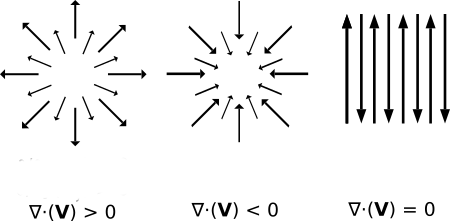
\includegraphics{figs/div.png}
  \caption{Ilustrația geometrică a divergenței}
  \label{fig:div}
\end{figure}

Similar, divergența se poate calcula și într-un punct, evaluînd toate calculele
din definiție într-un punct particular $ M(x_0, y_0, z_0) $.

Observăm, de asemenea, că:
\[
  \nabla \cdot \ : \text{ scalar sau vector } \mapsto \text{ scalar }.
\]

Vom mai folosi următorul concept:
\begin{definition}\label{def:solenoidal}\index{cîmp!solenoidal}
  Un cîmp vectorial $\vec{v} $ se numește \emph{solenoidal} în $ D $ dacă
  $ \nabla \cdot \vec{v} = 0 $ în $ D $.
\end{definition}

Intuitiv, un cîmp vectorial solenoidal este un cîmp fără surse, atît pozitive
(i.e.\ \qq{emisie}), cît și negative (i.e.\ \qq{absorbție}).

\vspace{1cm}
\index{cîmp!rotor}
Un al treilea operator care se poate aplica unui cîmp este \emph{rotorul}
(eng.\ \emph{curl}). Acesta este definit prin \emph{produsul vectorial} între
operatorul $ \nabla $ și cîmpul dat. Fie, deci, $ f : D \seq \RR^3 \to \RR $
un cîmp. Se definește:
\[
  \dr{rot}f = \nabla \times \vec{f} = %
  \begin{vmatrix}
    \vec{i} & \vec{j} & \vec{k} \\
    ?_x & ?_y & ?_z \\
    f & f & f
  \end{vmatrix},
\]
unde am folosit explicitarea produsului vectorial ca un determinant formal.

Continuînd calculele, obținem:
\[
  \nabla \times \vec{f} = (f_y - f_z, f_z - f_x, f_x - f_y).
\]

Observăm că rezultatul este un vector.

De cele mai multe ori, rotorul se aplică unui \emph{cîmp vectorial}, însă,
cînd componentele sînt diferite. Deci fie cîmpul vectorial:
\[
  \vec{V} : \RR^3 \to \RR^3, \quad \vec{V} = (V_1, V_2, V_3), \quad V_i : \RR^3 \to \RR.
\]

De exemplu, cum am întîlnit în capitolul anterior:
\[
  \vec{V} = (2x - 3y, 5x^2, z + 2x).
\]

Atunci rotorul se calculează:
\[
  \nabla \times \vec{V} = %
  \begin{vmatrix}
    \vec{i} & \vec{j} & \vec{k} \\
    ?_x & ?_y & ?_z \\
    V_1 & V_2 & V_3
  \end{vmatrix}
\]

Intuitiv, rotorul calculează gradul de \qq{rotație} al unui cîmp vectorial. De exemplu,
în cazul unui cîmp liniar, rotorul este nul, iar în cazul unui cîmp de tipul celui
magnetic sau gravitațional terestru, rotorul este nenul. Similar, putem gîndi cîmpul
dat de vînturi în cazul unui ciclon sau tornade. Rotorul acestui cîmp este nenul și,
în funcție de intensitatea fenomenului, modulul vectorului rotor într-un punct
este mai mare sau mai mic.

Un alt exemplu îl constituie \emph{cîmpurile solenoidale}, i.e.\ cele produse
de trecerea curentului electric printr-un solenoid. Din motive fizice evidente,
cîmpurile solenoidale au rotor nenul.

Cel mai adesea, avem, deci:
\[
  \nabla \times \ : \text{ vector } \mapsto \text{ vector }.
\]

De asemenea, avem definiția distinctă:
\begin{definition}\label{def:irot}\index{cîmp!irotațional}
  Cîmpul vectorial $ \vec{v} $ se numește \emph{irotațional} dacă $ \nabla \times \vec{v} = 0 $.
\end{definition}

Mai amintim că s-a studiat la calcul diferențial operatorul \emph{laplacian}. Dacă
$ f : D \seq \RR^3 \to \RR $ este un cîmp scalar, atunci se definește:
\[
  \Delta f = f_{xx} + f_{yy} + f_{zz}.
\]

\begin{remark}\label{rk:lapl-vec}
  Operatorul lui Laplace are sens și pentru un cîmp vectorial $ \vec{v} $, cu aceeași
  definiție.
\end{remark}

\textbf{Exercițiu*:} Arătați că $ \Delta f = \nabla \cdot (\nabla f) $, adică
laplacianul este divergența gradientului.

Rezultă, de asemenea:
\[
  \Delta \ : \text{ scalar } \mapsto \text{ scalar}.
\]

\vspace{1cm}

Cîteva identități care leagă operatorii definiți mai sus, precum și reguli de
calcul pot fi găsite de exemplu, \href{https://en.wikipedia.org/wiki/Vector\_calculus\_identities#Properties}{aici}.

\vspace{1cm}

Alte noțiuni utile sînt:
\begin{definition}\label{def:pot}\index{cîmp!potențial}
  Un cîmp vectorial $\vec{v} $ definit pe $ D \seq \RR^3 $ se numește \emph{potențial} dacă
  există un cîmp scalar $ f \in \kal{C}^1(D)$ cu proprietatea că:
  \[
    \vec{v}(M) = (\nabla f)(M), \quad \forall M \in D.
  \]
  Cîmpul scalar $ f $ se numește \emph{potențialul scalar} al cîmpului vectorial $ \vec{v} $.
\end{definition}

\begin{definition}\label{def:cons-forte}\index{cîmp!conservativ de forțe}
  Cîmpul vectorial $ \vec{F} $ se numește \emph{cîmp conservativ de forțe} dacă
  există un cîmp scalar $ U \in \kal{C}^1(D) $ astfel încît $ \vec{F} = \nabla U $.

  Altfel spus, un cîmp potențial provine dintr-un gradient, de aceea se mai numește
  \emph{cîmp de gradienți}.

  Cîmpul scalar $ U $ se numește \emph{cîmpul funcțiilor de forță}.
\end{definition}

De exemplu, cîmpul gravitațional este un cîmp conservativ de forțe. Ați întîlnit deja
în liceu noțiunea de \emph{forță conservativă} (al cărui lucru mecanic nu depinde de
forma traiectoriei, ci doar de capete) și, evident, cîmpul gravitațional este un cîmp
de forțe.


\begin{remark}\label{rk:cons-irot}
  Din definiția și proprietățile operatorilor vectoriali, un cîmp conservativ
  este în mod necesar irotațional.
\end{remark}

%%%%%%%%%%%%%%%%%%%%%%%%%%%%%%%%%%%%%%%%%%%%%%%%%%%%%%%%%%%%%%%%%%%%%%

\section{Exerciții}

1. Fie cîmpul scalar:
\[
  \varphi(x, y, z) = 2x^3 - 3y^2 + 6xyz.
\]

\begin{enumerate}[(a)]
\item Să se determine valoarea cîmpului $ \varphi $ în punctul $ A(1, -1, 0) $ și
  suprafața de nivel care trece prin punctul dat $ A $.
\item Să se determine derivatele funcției $ \varphi $ în punctul $ A $ după direcțiile
  axelor de coordonate și după direcția vectorului $ \vec{v} $, care unește punctul
  $ A $ cu punctul $ B(4, -2, 3) $.
\end{enumerate}

\vspace{1cm}

2. Fie cîmpul scalar $ \varphi(x, y, z) = x^2 + y^2 + z^2 $.
\begin{enumerate}[(a)]
\item Să se calculeze $ \nabla \varphi $;
\item Să se calculeze derivata cîmpului scalar $ \varphi $ după direcția vectorului
  $ \vec{s} = \dfrac{\vec{i} + \vec{j} + \vec{k}}{\sqrt{3}} $.
\end{enumerate}

\vspace{1cm}

3. Să se calculeze derivata cîmpului vectorial:
\[
  \vec{v} = (y + xz)\vec{i} + (x + yz) \vec{j} + (x^2 - y^2) \vec{k}
\]
după direcția vectorului $ \vec{u} = \vec{i} + 2 \vec{j} + 2 \vec{k} $.

\emph{Indicație:} Dacă notăm $ \vec{v} = (v_1, v_2, v_3) $, atunci se calculează
derivatele acestor componente după direcția $ \vec{u} $, adică $ \vec{u} \cdot \nabla v_{1,2,3} $.

\vspace{1cm}

4. Fie cîmpurile:
\begin{align*}
  \vec{v} &= (xyz + x^3) \vec{i} + (y^2 + y^3) \vec{j} + (xz^2 + z^3) \vec{k} \\
  \vec{w} &= (yz + xy^2) \vec{i} + (xyz + yz^2) \vec{j} + (3xy + x^2 z) \vec{k}.
\end{align*}

Să se calculeze $ \nabla(\nabla \cdot \vec{v}) $ și $ \nabla \times (\nabla \times \vec{w}) $.

\vspace{1cm}

5. Fie cîmpul scalar:
\[
  f(x, y, z) = \dfrac{\langle \vec{a}, \vec{r} \rangle}{||\vec{r}||^2}, \quad \text{unde } %
  \vec{a} = 2 \vec{i} + \vec{j} - \vec{k}, \ \vec{r} = x\vec{i} + y\vec{j} + z \vec{k}.
\]

Să se calculeze unghiul dintre $ (\nabla f)(A) $ și $ (\nabla f)(B) $, unde
$ A(2, 1, 1) $ și $ B(0, 1, -1) $.

\emph{Indicații:} Fie $ M(x, y, z) $ oarecare. Se calculează $ (\nabla f)(M) $ folosind
regula de calcul a gradientului unei fracții și se obține:
\[
  (\nabla f)(M) = \dfrac{\vec{a}}{||\vec{r}||} - 2 \cdot \dfrac{\langle \vec{a}, \vec{r} \rangle}{||\vec{r}||^4} %
  \cdot \vec{r}.
\]

Atunci putem calcula în punctele $ A $ și $ B $ date, iar unghiul va fi obținut din:
\[
  \cos \theta = \dfrac{\langle (\nabla f)(A), (\nabla f)(B) \rangle}{%
    ||(\nabla f)(A)|| \cdot || (\nabla f)(B) ||}.
\]

Se obtine $ \cos \theta < 0 $, deci unghiul este obtuz, cu o valoare de $ \arccos -\dfrac{5}{9} $.


%%% Local Variables:
%%% mode: latex
%%% TeX-master: "../edtc-18-19"
%%% End:
